% !TEX root = ../main.tex
%
\section{Introduction}
\label{sec:introduction}

The modern social media environment has evolved to be extremely demanding, with users of social networks facing ever-increasing threats such as targeted misinformation \cite{clemons2025disinformation, Denniss2025Social}, hate speech \cite{kolluri2025parler}, and polarization \cite{pranesh2024impactsocialmediapolarization}. These threats can cause serious emotional and mental harm \citep{proactive_moderation}, radicalization \citep{cho-etal-2024-language}, real-world violence \citep{schaffner_community_guidelines}, as well as sabotage democratic dialogue \citep{esau2017design, falk-etal-2021-predicting, seering_self_moderation}, trust in democratic institutions \citep{schroeder-etal-2024-fora} and quality of information \citep{make_reddit_great}. Platform designers and researchers traditionally focused on flagging and removing problematic content (``content moderation'' --- \citet{seering_self_moderation, cresci_pesonalized_interventions}), but these methods are no longer sufficient in practice \cite{horta_automated_moderation, schaffner_community_guidelines, small-polis-llm, korre2025evaluation}. Instead, online communities are at their best when moderators actively discuss and explain their actions (``conversational moderation'' or ``facilitation'' --- \citet{argyle2023, korre2025evaluation, falk-etal-2021-predicting}); thus preventing problematic user behavior before it surfaces \cite{cho-etal-2024-language, seering_self_moderation, cresci_pesonalized_interventions, make_reddit_great}, as well as supporting community deliberation and group decision-making \cite{kim_et_al_chatbot, seering_self_moderation}. 

\begin{figure}[t]
	\centering
	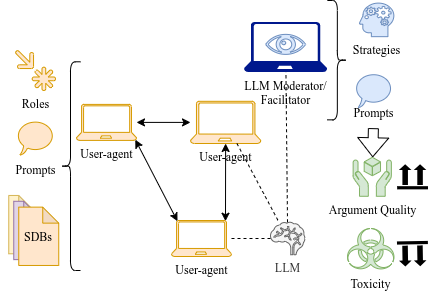
\includegraphics[width=\columnwidth]{research_goal.png}
	\caption{LLM user-agents with distinct SocioDemographic Backgrounds (SDBs) participate in a discussion, while the LLM moderator monitors and attempts to improve the quality of the discussion. We need to design prompts and configurations for both types of LLM agents.}
	\label{fig::goals}
\end{figure}

Large Language Models (LLMs) have been hypothesized to be capable of facilitation tasks and can be scaled to a far greater extent compared to human facilitators \cite{korre2025evaluation, small-polis-llm}, making them a viable choice for modern large-scale social networks. However, experimentation and development on these systems is hampered due to the costs of human participation---in this case, human discussants and evaluators \citep{rossi_2024}. We posit that simulations with all-LLM-agents can be a cheap and fast way to develop and test LLM facilitators, initial versions of which may be unstable or unpredictable \cite{atil_2025, rossi_2024}, before testing them with human participants. 

Our work asks the following research question: \emph{How do we design and evaluate Synthetic Discussion Generation (SDG) methodologies satisfying registered criteria}? To answer this question we draw examples from methodologies proposed in literature, to establish basic design principles (\S\ref{ssec:methodology:design}), and we propose a methodology enabling rapid model ``debugging'' (e.g., discarding suboptimal LLM prompts) and testing without human involvement (Fig.~\ref{fig::goals}, \S\ref{ssec:methodology:us}). We validate the outcome through an ablation study (\S\ref{ssec:results:ablation}). To show the impact of our approach, we implement a framework based on the proposed methodology, which allows the design and evaluation of facilitation strategies proposed in modern Social Science research. Then, we investigated how they can enhance the performance of LLM facilitators. We compare them with two common facilitation setups (\S\ref{ssec:experimental:strategies}) and find that while the presence of LLM facilitators has a \emph{positive, statistically significant} influence on the quality of synthetic discussions, facilitation strategies inspired by Social Science research often \emph{do not outperform simpler strategies} (\S\ref{ssec:results:main}). We also discover previously unreported aberrant behavior on the part of the LLM facilitator, in the form of excessive policing.

Finally, we release an open-source Python framework, available via PIP, that implements our methodology at scale, enabling the research community to rapidly experiment with LLM-based facilitators. Given that existing facilitation datasets are few and generally small \citep{korre2025evaluation}, we also release \vmd a large, publicly available dataset with LLM-generated and annotated synthetic discussions (\S\ref{sec:data-soft}). Our dataset can be used for LLM facilitator finetuning \cite{ulmer2024}, as well as for analyzing the behavior of out-of-the-box LLMs in the task of online facilitation. We use open-source LLMs and include all relevant configurations in order to make our study as reproducible as possible.
